Analog-to-Digital Converter (ADC) are electronic devices that can convert analog voltage signals to digital values, as shown in \autoref{fig:Conversion_AD_DA}. They imply a resolution $R_{ADC}$ and a dynamic range that limit the final precision of the instrument \cite{horowitz1989art}. The ADC converts analog continuous values into digitized ones that follow quantized steps such as those illustrated in \autoref{fig:ADC_voltage_resolution}. The resolution  $R_{ADC}$ of the ADC thus depends on the Effective Number Of Bits ($ENOB$)\cite{leHuy2004circuits} of the system, which is a practical measure of its resolution that takes into consideration the system’s noise floor and the Full Scale Voltage Range $E_{FSR}$ of the power-supplies $V_{DD}$ and $V_{SS}$ (or $V_{RefHi}$ and $V_{RefLo}$, respectively) of the ADC:
\begin{equation}
   R_{ADC} = E_{FSR} (\frac{1}{2})^{ENOB}
\end{equation}
\begin{equation}
   E_{FSR} = (V_{DD}-V_{SS})
\end{equation}
\begin{figure}[h]
    \centering
    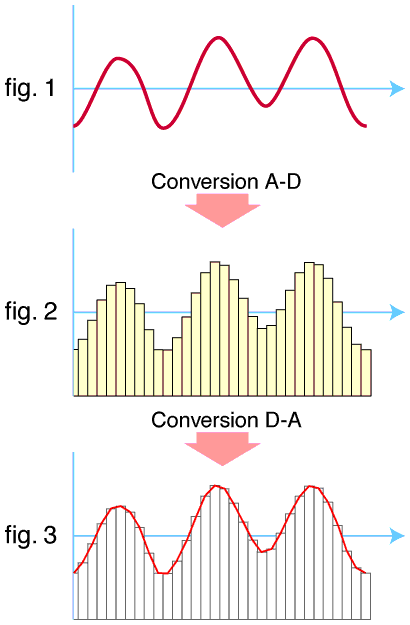
\includegraphics[width=0.4\textwidth]{Conversion_AD_DA}
    \caption{Conversion from the analog (A) domain to the digital (D) domain, followed by a reconstruction in the analog domain.}
    \label{fig:Conversion_AD_DA}
\end{figure}
The $ENOB$ is always slightly lower than the ideal binary dynamic range of the ADC expressed by its number of bits. For a hypothetical 10-bit ADC with an $ENOB$ of 9.5 linked to a unipolar power-supply of 3.3 V, the minimum voltage step would be 4.56 mV. \par
\begin{figure}[h]
    \centering
    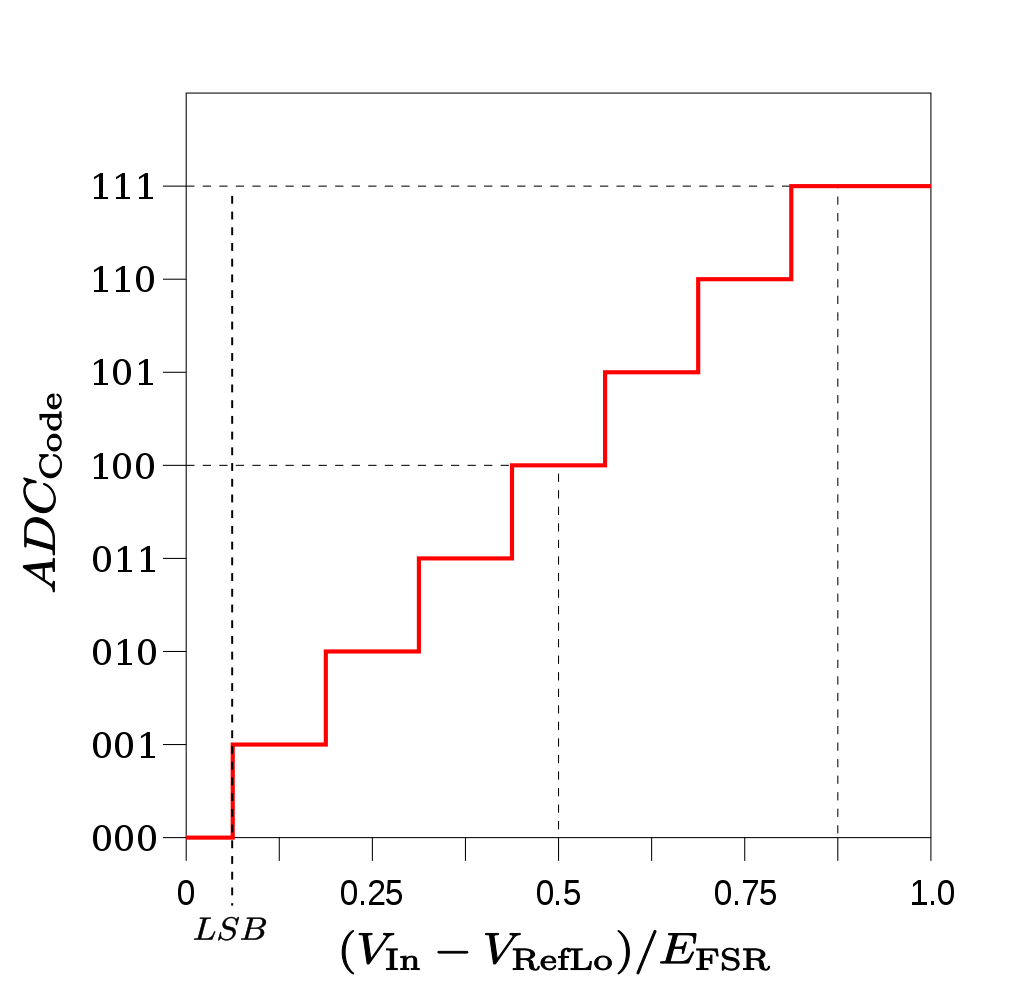
\includegraphics[width=0.6\textwidth]{ADC_voltage_resolution}
    \caption{Resolution increments of a 3-bits ADC.}
    \label{fig:ADC_voltage_resolution}
\end{figure}